\subsection{Normalized Step Response}
In this section, the normalized step response on the two controlled variabels ($u$) is seen. The step response is determined by first step on $u_1$ and the result is evaluated at the height in tank 1 and 2 (as seen on the left column of \cref{fig:norm_step}) at the 3 step amplitudes (10, 25 and 50\%). Afterwards the same is done for $u_2$ (as seen on the right column of \cref{fig:norm_step}). During the simulation, the disturbance is kept constant at $250\,[cm^3/s]$.
\begin{figure}[H]
    \centering
    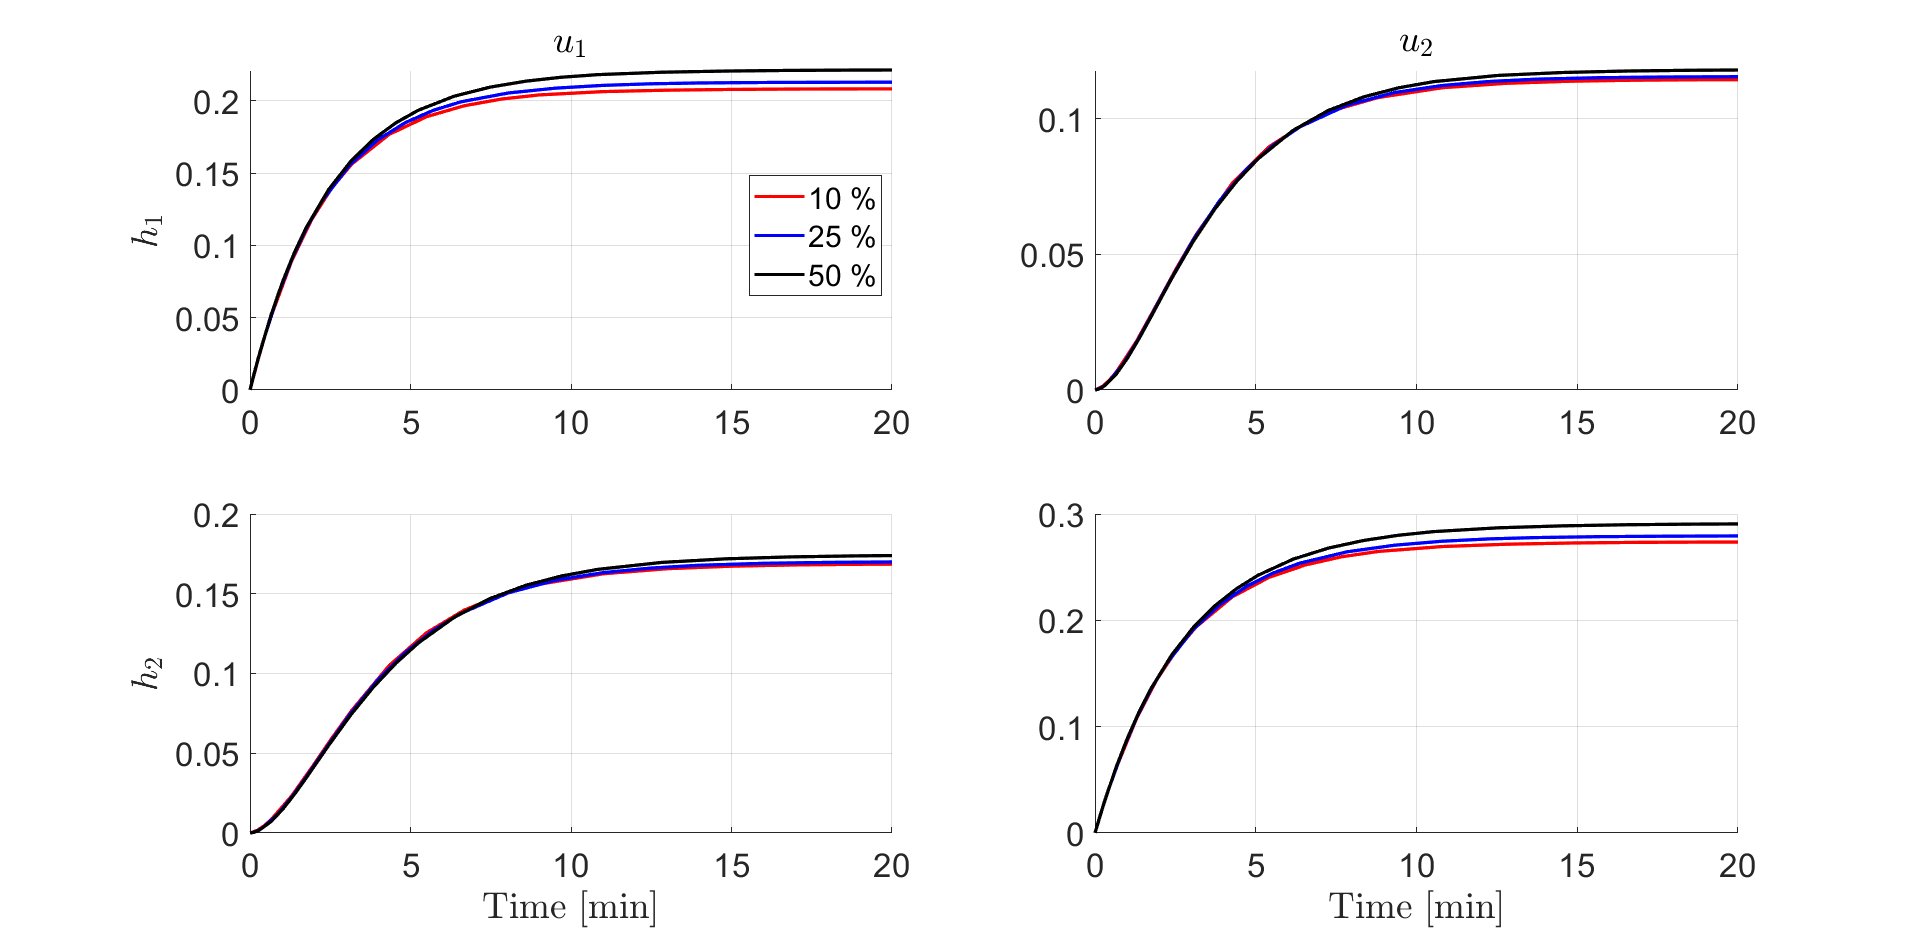
\includegraphics[width=1\textwidth]{Figures/Pr3.3_Norm_Step.png}
    \caption{Normalized step response - Deterministic model}
    \label{fig:norm_step}
\end{figure}
It is seen that the normalized step on each of the inputs are not the same, which is due to the non-linearity of the system. If the system was linear, the responses would be similar.\\
Similar to the deterministic system, the normalized step for the stochastic system is evaluated. In the given case, only the outputs relating to the input 1 is shown where the low noise level is used (see \cref{eq:Noise_values}).
\begin{figure}[H]
    \centering
    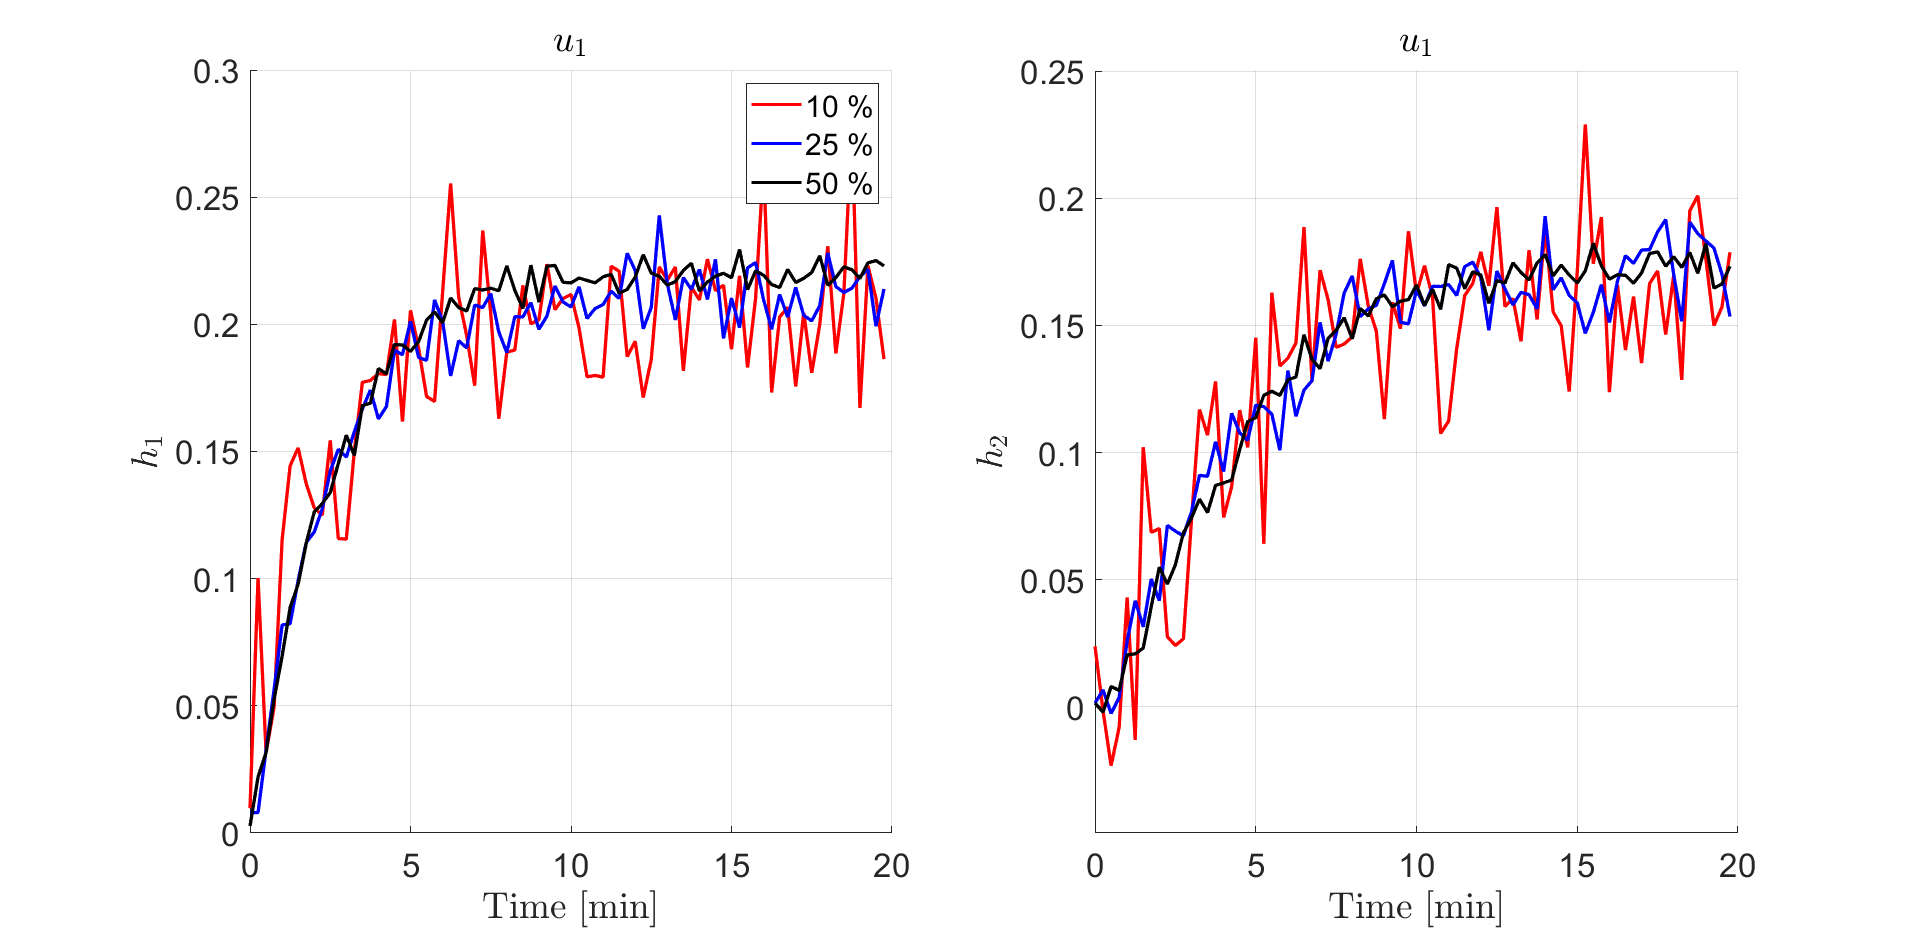
\includegraphics[width=1\textwidth]{Figures/Pr3.3_Norm_Step_Stoc.png}
    \caption{Normalized step response - Stochastic model}
    %\label{fig:norm_step}
\end{figure}
It is seen the stochastic model follows the same response as the deterministic system. However the noise is clearly present. Since the noise has a larger relative influence on the system with small steps (10\%) than it has on the system with large steps (50\%), the noise seems larger for the small steps. 